\documentclass[journal]{IEEEtran}
\usepackage{graphicx}
\usepackage{amsmath,amssymb}
\usepackage{booktabs,array}
\usepackage{url}
\usepackage{cite}
\usepackage{balance}
\title{PG-CARE: Leakage-Free Physics-Guided Conformal Reliability for One-Hour-Ahead EV Flexibility Forecasting and Distribution-Feeder Support}
\author{Mahmoud M. Kiasari and Hamed H. Aly%
\thanks{The authors are with the Department of Electrical and Computer Engineering, Dalhousie University, Halifax, NS, Canada.}}
\begin{document}
\maketitle
\begin{abstract}
Reliable vehicle-to-grid (V2G) operation requires more than accurate electric-vehicle (EV) state classification: a forecast must be issued without access to target-time information, remain physically feasible, quantify uncertainty, and create useful feeder support when the realized fleet differs from expectation. This paper presents PG-CARE, a model-agnostic reliability envelope for one-hour-ahead EV operating-state and flexibility forecasting. The study reconstructs the supervisory logic of a previously published MATLAB/Simulink controller in a scalable Python digital twin with 100 heterogeneous EVs, 365 days, and 3.504 million EV-time states. A critical leakage pathway is removed by separating owner-declared connection schedules from realized future connectivity and forecasting the latter only from information available at issuance time. On the full 85-day chronological test interval (203,900 hourly forecasts), raw LightGBM achieves 0.7986 macro-F1 and 0.6700 V2G F1. Leak-free feasibility projection raises these to 0.8140 and 0.7088, while conformal abstention reaches 0.8183 and 0.7155. A paired issue-time block bootstrap gives a macro-F1 improvement of +0.0196 with a 95\% confidence interval of [0.0171,0.0221]. A separate future-connectivity predictor achieves 0.9702 accuracy and 0.9960 ROC-AUC. Conformalized quantile regression (CQR) provides 0.8996 empirical coverage for upward flexibility. Balanced AC quasi-static time-series analysis on the IEEE 33-bus feeder shows the reliability-value tradeoff: raw mean flexibility supplies stronger feeder support but incurs 8.678 MWh of commitment shortfall, whereas conservative CQR and reliability-budgeted recovery (RBR) policies produce zero observed shortfall while recovering part of the feeder benefit. Marginal state-set coverage is 0.9117, but V2G conditional coverage is only 0.8016, which is reported as a limitation rather than hidden.
\end{abstract}
\begin{IEEEkeywords}
Electric vehicles, vehicle-to-grid, conformal prediction, flexibility forecasting, physical feasibility, uncertainty quantification, distribution feeder, quasi-static time series.
\end{IEEEkeywords}

\begin{figure*}[t]
\centering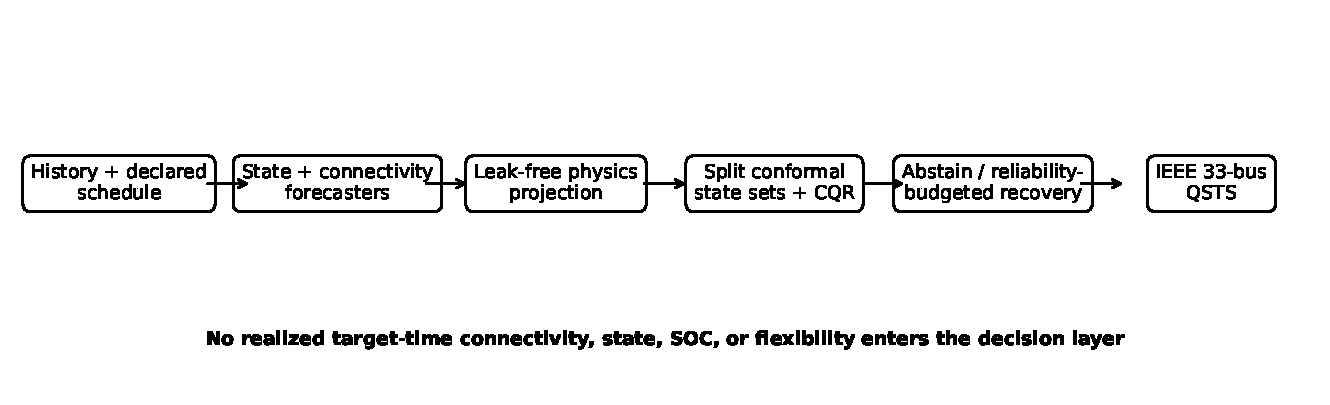
\includegraphics[width=0.96\textwidth]{../figures_v2/fig1_v2_framework.pdf}
\caption{PG-CARE v2 information flow. Realized target-time connectivity, state, SOC, and flexibility are prohibited from the decision layer.}
\label{fig:framework}
\end{figure*}

\section{Introduction}
EV aggregators can transform flexible charging loads into controllable grid resources, but the value of that flexibility depends on whether it is still available when a scheduling or reserve decision is executed. Recent work has therefore moved from deterministic charging schedules toward aggregate flexibility, stochastic model predictive control, user-aware scheduling, safe reinforcement learning, and distribution-network-aware flexibility representations \cite{r12,r17,r18,r26,r27,r28,r29,r37,r38,r39}. In parallel, EV load forecasting has adopted multi-scale expert systems, spatio-temporal graph models, causal generalization mechanisms, and value-oriented training \cite{r11,r19,r20,r21,r22,r30,r40}. These developments raise a stricter question than which model has the highest accuracy: can a forecast be trusted enough to authorize a physical V2G commitment?

The authors' earlier MATLAB/Simulink work \cite{r1} established owner participation choices, minimum-SOC protection, V2G/G2V/Idle supervisory logic, and a bidirectional charger-oriented controller. Its four-EV/four-household scale was adequate for controller demonstration but not for statistical forecasting. A subsequent large-scale forecasting formulation exposed a second problem: a physical mask that uses realized future connectivity can silently leak target-time information into the classifier. This paper treats removal of that leak as a design requirement rather than a cosmetic revision.

PG-CARE is positioned as a reliability envelope around a forecasting backbone, not as a claim that a particular deep architecture dominates all alternatives. It separates declared schedule information from realized connectivity; predicts future connectivity explicitly; projects state probabilities through feasibility rules using issuance-time information only; calibrates state prediction sets and flexibility intervals after the projection; and allows the controller to abstain or recover flexibility according to a validation-selected reliability budget. Feeder-level QSTS then measures the operational consequence of conservative versus aggressive commitments.

The contributions are: 1) a leak-free information structure with an automated source-code invariant test; 2) split-conformal state sets and CQR flexibility intervals calibrated after physics projection; 3) reliability-budgeted recovery (RBR) that recovers part of a conservative lower-bound commitment under validation constraints; and 4) full chronological, rolling-origin, unseen-EV, schedule-stress, block-bootstrap, and IEEE 33-bus feeder validation.

\section{Related Work and Positioning}
\subsection{EV flexibility and grid services}
Modern EV aggregation studies increasingly model flexibility as a bounded, uncertain resource. Learning-based aggregate flexibility \cite{r12}, population envelopes \cite{r17}, stochastic reserve provision using more than one million charging records \cite{r18}, user-anxiety-aware frequency regulation \cite{r26}, carbon-aware flexibility \cite{r27}, hierarchical disaggregation feasibility \cite{r28}, and heterogeneous renewable-following flexibility \cite{r29} emphasize both power and energy feasibility. Analytical polytope aggregation has been demonstrated on IEEE 33- and 141-bus networks \cite{r37}, while degradation cost materially changes the usable fleet region \cite{r38}.

\subsection{Forecasting, generalization, and uncertainty}
Current forecasting work includes multi-scale spatial-temporal GNNs \cite{r11}, deep expert systems \cite{r19}, causal generalization \cite{r22}, robust adaptive uncertainty sets \cite{r25}, stacked meta-learning for EV load \cite{r30}, and 2026 highway forecasting with independent scenarios \cite{r40}. Value-oriented forecasting shows that operational cost can rank forecasts differently from statistical error \cite{r20,r21}. Conformal prediction is increasingly used in energy applications \cite{r31,r32,r33,r34,r35}, but marginal validity does not imply conditional validity by class/hour or arbitrary distribution shift.

\section{Digital Twin and Leak-Free Forecasting Problem}
\subsection{Supervisory reconstruction}
The digital twin is a supervisory reconstruction of the concepts in \cite{r1}, not switching-level equivalence to the original 10-kHz converter. It models 100 heterogeneous EVs for 365 days at 15-min resolution, yielding 3,504,000 EV-time states. Battery SOC evolves as
\begin{equation}
SOC_{i,t+1}=SOC_{i,t}+\frac{(\eta_cP^c_{i,t}-P^d_{i,t}/\eta_d)\Delta t}{E_i}.
\end{equation}
Three symbolic states---G2V, Idle, V2G---are used to avoid historical sign-convention ambiguity.

\subsection{Declared versus realized connection}
Owner-declared arrival and departure are generated separately from realized connection. Late arrival, early departure, and timing noise create about 3.1\% one-hour-ahead declaration/realization mismatch. At forecast issuance time $t$, the model may use declaration and history through $t$, but not realized $a_{t+H}$.
\begin{figure}[t]\centering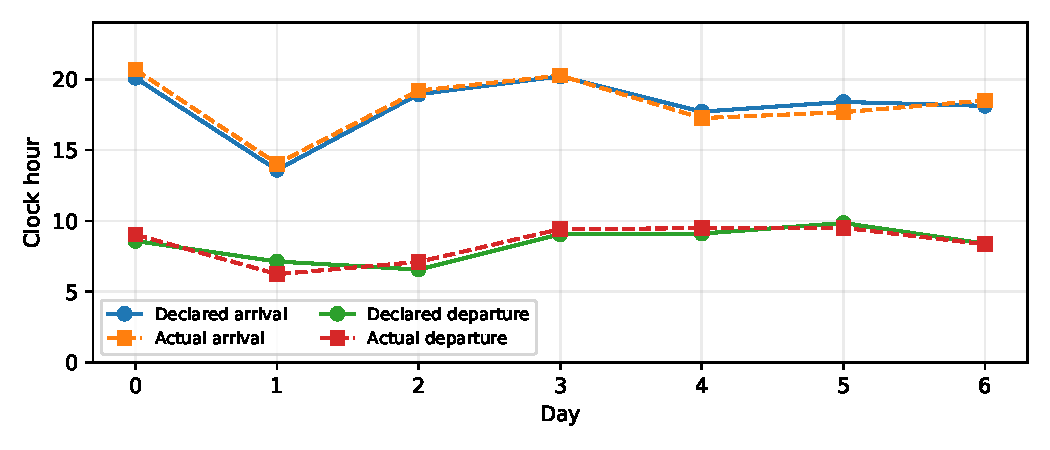
\includegraphics[width=\columnwidth]{../figures_v2/fig2_schedule_uncertainty.pdf}\caption{Declared and realized connection schedules are distinct.}\label{fig:sched}\end{figure}

The horizon is $H=1$ h and history length is $L=2$ h. Outputs include the target state, target connectivity probability, and upward flexibility. The final test issues forecasts once per hour for all 100 EVs across 85 days, producing 203,900 examples without random test subsampling.

\section{Information-Safe Problem Formulation}
Let $\mathcal I_t$ denote all information available at forecast issuance: observations through $t$, declared schedules, static parameters, and exogenous inputs known or forecast at $t$. It excludes realized target-time connectivity, state, SOC, and flexibility. Every deterministic pre-decision transformation must be a function of $\mathcal I_t$ only.

The raw state probabilities $\hat{\mathbf p}$ are projected by a deterministic feasible mask $\mathbf m(\mathcal I_t)$,
\begin{equation}
\tilde p_k=\frac{m_k\hat p_k}{\sum_jm_j\hat p_j},
\end{equation}
with Idle as the safe fallback. A binary LightGBM future-connectivity model provides $\hat a_{t+H}$ rather than using the realized connection. It achieves 0.9702 accuracy, 0.9722 F1, and 0.9960 ROC-AUC on the chronological test set.

\section{PG-CARE Reliability Envelope}
\subsection{Split-conformal state sets}
The class nonconformity score is $s(x,y)=1-\tilde p_y(x)$. Using calibration size $n$, the finite-sample split-conformal quantile is selected and
\begin{equation}
\Gamma_\alpha(x)=\{k:1-\tilde p_k(x)\le q_\alpha\}.
\end{equation}
A state decision is authorized only when the set is singleton and feasible; otherwise the system abstains to a conservative fallback.

\emph{Proposition 1 (marginal post-projection validity):} If the projection is a deterministic measurable function of issuance-time information only and calibration/test pairs are exchangeable, then calibrating the conformal score after the projection preserves the standard split-conformal marginal coverage guarantee. This statement does not imply class-conditional, hour-conditional, or arbitrary time-series/OOD coverage.

\subsection{CQR flexibility and RBR}
LightGBM point and quantile regressors estimate upward flexibility. CQR produces a calibrated interval $[L_t,U_t]$. A strict commitment $L_t^+=\max(0,L_t)$ is safe but conservative. RBR uses
\begin{equation}
P_t^{\rm RBR}=L_t^+ + \beta g_t\max(0,\hat P_t^{up}-L_t^+),
\end{equation}
where $g_t\in[0,1]$ decreases with interval width and is enabled only for singleton state sets with sufficiently high predicted connectivity. $\beta$ is selected on validation data under a preset committed-flexibility shortfall budget and is never tuned on test data.

\section{Experimental Protocol}
Days 1--200 are used for fitting, 201--240 for conformal calibration, 241--280 for validation/decision tuning, and 281--365 for the untouched test. State metrics include accuracy, balanced accuracy, macro-F1, MCC, and per-class F1. Calibration is assessed using ECE, multiclass Brier score, marginal and conditional coverage, and set size. Regression uses MAE/RMSE and CQR coverage/width. Statistical uncertainty uses 1,000 paired block-bootstrap resamples over forecast issue times.

Generalization tests include training on EVs 0--79 and testing on never-seen EVs 80--99, feature-group ablation, 12\% declared-connectivity corruption plus time-to-departure jitter, and rolling-origin 14-day test blocks.

A balanced AC backward/forward-sweep implementation of the standard IEEE 33-bus radial feeder evaluates five strategies across all 2,039 hourly test instants: no forecast V2G, raw mean flexibility, CQR lower bound, RBR, and oracle realized flexibility. The feeder is deliberately stressed and is used as a relative benchmark, not a utility-specific operating study.

\section{Results}
\subsection{Leak-free state forecasting}
\begin{table}[t]\centering\caption{Full 85-Day Chronological Test}\label{tab:cls}\resizebox{\columnwidth}{!}{\begin{tabular}{lccccc}\toprule Method&Acc.&Bal. Acc.&Macro-F1&MCC&V2G F1\\\midrule LightGBM raw&0.9088&0.8905&0.7986&0.7303&0.6700\\ Leak-free physics&0.9160&0.8824&0.8140&0.7421&0.7088\\ PG-CARE v2&0.9186&0.8785&0.8183&0.7459&0.7155\\\bottomrule\end{tabular}}\end{table}
Removing target-time connectivity reduces the physics benefit to a credible magnitude. A paired issue-time block bootstrap gives $\Delta$macro-F1=+0.0196 with 95\% CI [0.0171,0.0221] and $\Delta$MCC=+0.0155 with CI [0.0130,0.0179]. Exact McNemar testing finds 2,554 raw errors corrected by PG-CARE versus 543 cases degraded ($p\approx6.26\times10^{-310}$), while the block bootstrap is emphasized because EVs sharing an issue time are dependent.
\begin{figure}[t]\centering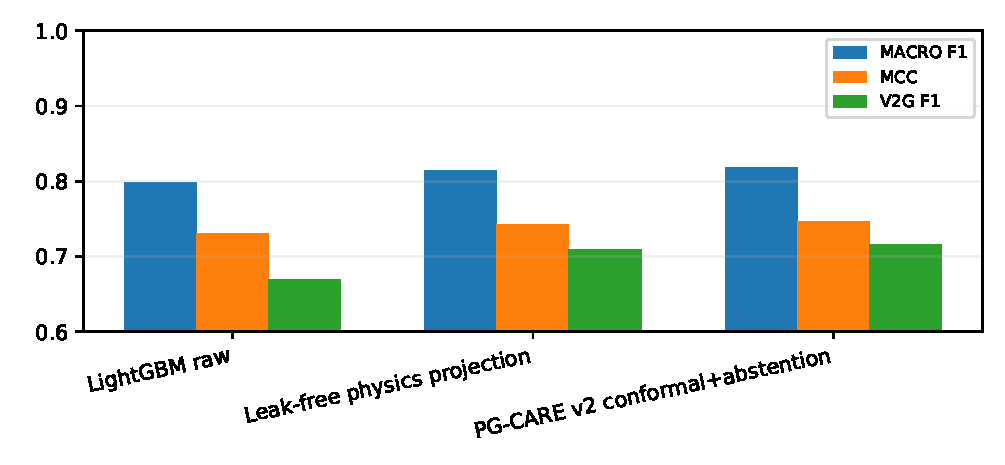
\includegraphics[width=\columnwidth]{../figures_v2/fig3_leakfree_metrics.pdf}\caption{Leak-free classification performance.}\label{fig:metrics}\end{figure}

PG-CARE improves macro-F1 in every rolling block. On unseen EVs, macro-F1 is 0.7857 and V2G F1 is 0.6484. With 12\% schedule corruption these become 0.7766 and 0.6221. Removing static identity features lowers unseen-EV macro-F1 from 0.7808 to 0.7541, while removing the declared schedule lowers it to 0.7177.
\begin{figure}[t]\centering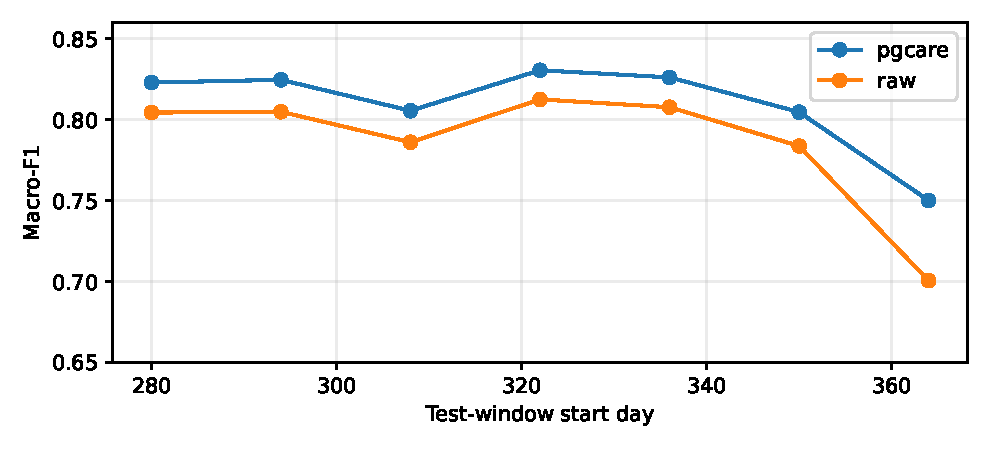
\includegraphics[width=\columnwidth]{../figures_v2/fig4_rolling_origin.pdf}\caption{Rolling-origin macro-F1.}\label{fig:roll}\end{figure}
\begin{figure}[t]\centering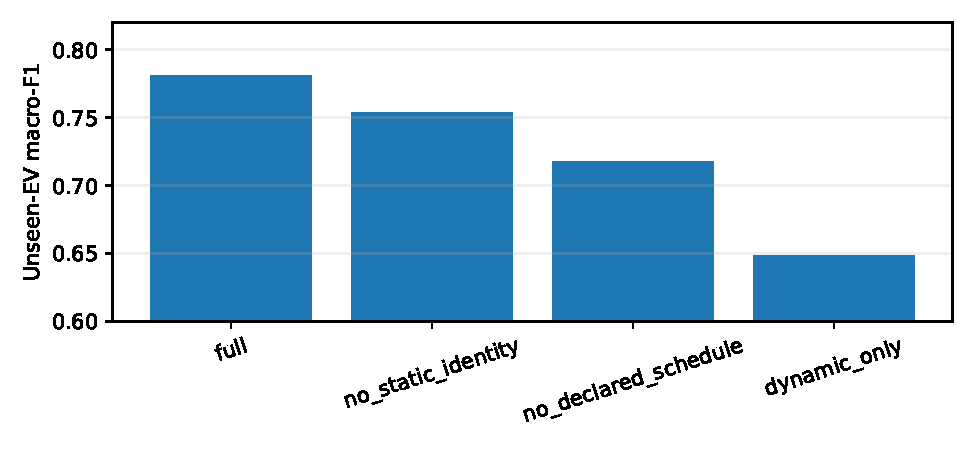
\includegraphics[width=\columnwidth]{../figures_v2/fig5_feature_ablation.pdf}\caption{Unseen-EV feature-group ablation.}\label{fig:abl}\end{figure}

\subsection{Calibration and flexibility intervals}
Projected probabilities reduce multiclass Brier score from 0.1311 to 0.1215 but increase ECE from 0.0201 to 0.0289. State sets achieve 0.9117 marginal coverage at nominal 0.90 with mean set size 0.9906. Coverage is not uniform: Idle=0.9172, G2V=0.9079, and V2G=0.8016. The 00:00--04:00 block is 0.8348. These failures prohibit a stronger conditional-validity claim.
\begin{figure}[t]\centering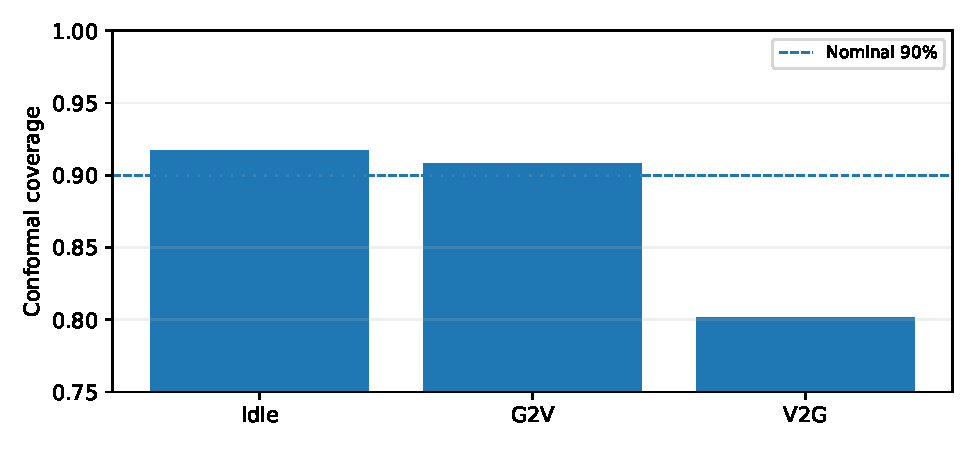
\includegraphics[width=\columnwidth]{../figures_v2/fig6_class_coverage.pdf}\caption{Class-conditional conformal coverage.}\label{fig:cov}\end{figure}
The upward-flexibility point predictor obtains 0.6828-kW MAE and 1.9207-kW RMSE. CQR obtains 0.8996 empirical coverage with 6.5018-kW mean width; 67.76\% of examples have a zero conservative lower bound.
\begin{figure}[t]\centering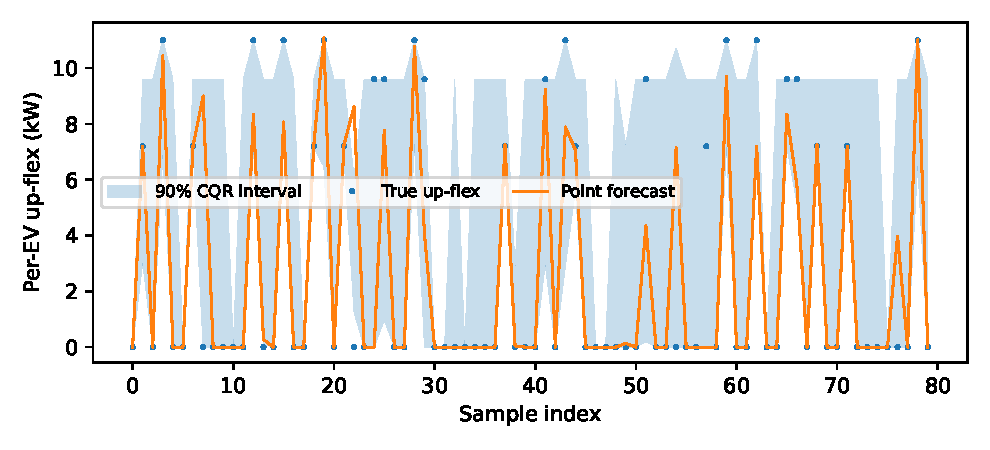
\includegraphics[width=\columnwidth]{../figures_v2/fig8_cqr.pdf}\caption{CQR intervals for upward flexibility.}\label{fig:cqr}\end{figure}

\subsection{IEEE 33-bus reliability-value tradeoff}
\begin{table*}[t]\centering\caption{IEEE 33-Bus QSTS Stress Test}\label{tab:qsts}\begin{tabular}{lrrrrrr}\toprule Strategy&Min V&Violation bus-steps&Loss (kW)&Peak (kW)&Delivered (MWh)&Shortfall (MWh)\\\midrule No forecast V2G&0.739&32700&270.4&11181&0.00&0.00\\ Oracle flexibility&0.747&32567&256.1&10778&152.18&0.00\\ PG-CARE CQR lower&0.740&32662&266.5&11089&43.13&0.00\\ PG-CARE RBR&0.741&32650&265.6&11060&53.76&0.00\\ Raw mean flexibility&0.746&32592&258.5&10849&125.54&8.68\\\bottomrule\end{tabular}\end{table*}
Raw mean flexibility is aggressive: it delivers 125.54 MWh and produces stronger voltage/loss/peak effects, but overcommits by 8.678 MWh. CQR lower delivers 43.13 MWh with zero observed shortfall. RBR increases delivered support to 53.76 MWh while retaining zero observed commitment shortfall in the test. Oracle flexibility defines the upper benchmark.
\begin{figure}[t]\centering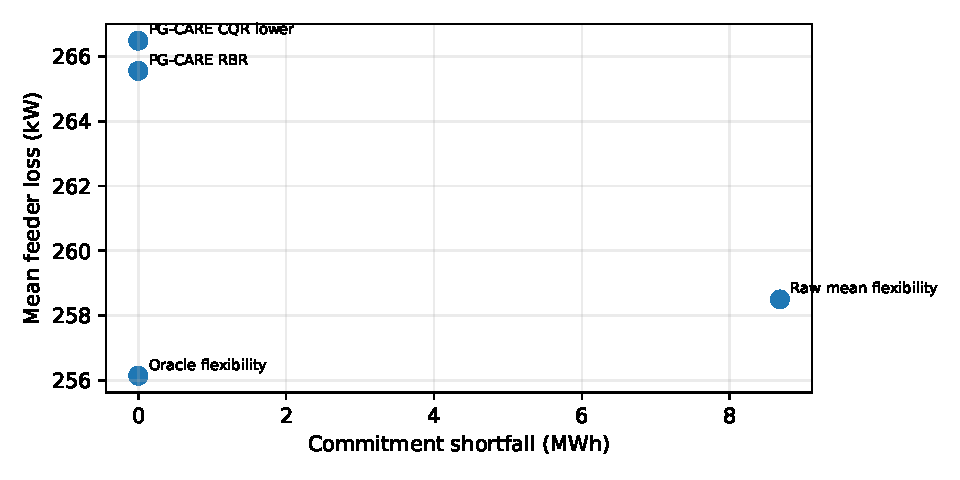
\includegraphics[width=\columnwidth]{../figures_v2/fig7_qsts_tradeoff.pdf}\caption{Reliability-value tradeoff on the feeder stress test.}\label{fig:qsts}\end{figure}

\section{Computational and Reliability Analysis}
The final connectivity and state models train in approximately 1.87 s and 7.82 s, respectively, on the recorded CPU environment. Deployment requires one connectivity probability, one state-probability vector, deterministic masking, a conformal lookup, and three flexibility regressors per forecast. The method is backbone-agnostic; future spatio-temporal or state-space models may replace the tree backbone without changing the information-integrity rules.

Three visible failure modes remain. First, V2G coverage is below nominal. Second, schedule corruption disproportionately harms V2G near availability/SOC boundaries. Third, the CQR lower bound is frequently zero, so reliable commitment is conservative. RBR addresses only the third issue empirically. The oracle gap is still large: RBR delivers 53.76 MWh versus 152.18 MWh with perfect realized flexibility.

\section{Discussion and Limitations}
The novelty is not LightGBM, a deterministic EV rule, conformal prediction, or IEEE 33-bus simulation in isolation. It is the information-safe composition: future availability is predicted rather than leaked; physical projection is restricted to issuance-time information; conformal classification and CQR are calibrated after that projection; abstention prevents unsupported commitments; and RBR maps interval width and forecast connectivity into a tunable reliability budget before a network action.

The revised classification gain is intentionally smaller than the earlier draft because the strongest apparent gain in that draft came from target-time connectivity inside the physical mask. Retaining that inflated result would be indefensible. The remaining gain is statistically stable and supports a feeder commitment layer that exposes the cost of overconfidence.

The present evidence remains a source-informed stochastic digital twin plus a standard test feeder. It is not a field trial, does not reproduce switching-level converter waveforms, and does not establish arbitrary OOD conformal validity. The stressed feeder voltages are useful for relative comparison rather than utility-specific absolute values. The package includes measured-data acquisition adapters for ACN-Data-style sessions and Open Power System Data household/PV traces, but external raw data are not redistributed or claimed as executed validation. External measured-data validation and improved V2G-conditional calibration are the two highest-priority steps before a final flagship submission.

\section{Reproducibility and Conclusion}
The archive contains the original Simulink artifact, Python twin, leak-free pipeline, frozen models, chronological results, full test predictions, block-bootstrap replicates, feeder QSTS code/results, vector figures, source-code invariant test, exact environment metadata, traceability files, and SHA-256 hashes.

PG-CARE v2 reframes one-hour-ahead EV forecasting as an information-integrity and decision-reliability problem. After eliminating future-connectivity leakage, feasible conformal decisions improve state reliability modestly but consistently, while CQR and RBR expose a clear reliability-value frontier for V2G commitment. The main unresolved result is equally important: nominal marginal coverage does not guarantee V2G conditional coverage, and external measured-data validation remains necessary before claiming field generalization.

\balance
\begin{thebibliography}{40}
\bibitem{r1} M. M. Kiasari and H. H. Aly, ``A proposed controller for real-time management of electrical vehicle battery fleet with MATLAB/SIMULINK,'' \emph{Journal of Energy Storage}, vol. 99, pp. 113235, 2024, doi: 10.1016/j.est.2024.113235.
\bibitem{r2} H. Jahangir, S. S. Gougheri, B. Vatandoust, M. A. Golkar, A. Ahmadian, and A. Hajizadeh, ``Plug-in Electric Vehicle Behavior Modeling in Energy Market: A Novel Deep Learning-Based Approach With Clustering Technique,'' \emph{IEEE Transactions on Smart Grid}, vol. 11, no. 6, pp. 4738-4748, 2020, doi: 10.1109/TSG.2020.2998072.
\bibitem{r3} Z. J. Lee et al., ``Adaptive Charging Networks: A Framework for Smart Electric Vehicle Charging,'' \emph{IEEE Transactions on Smart Grid}, vol. 12, no. 5, pp. 4339-4350, 2021, doi: 10.1109/TSG.2021.3074437.
\bibitem{r4} Z. J. Lee, S. Sharma, D. Johansson, and S. H. Low, ``ACN-Sim: An Open-Source Simulator for Data-Driven Electric Vehicle Charging Research,'' \emph{IEEE Transactions on Smart Grid}, vol. 12, no. 6, pp. 5113-5123, 2021, doi: 10.1109/TSG.2021.3103156.
\bibitem{r5} T. Long, Q.-S. Jia, G. Wang, and Y. Yang, ``Efficient Real-Time EV Charging Scheduling via Ordinal Optimization,'' \emph{IEEE Transactions on Smart Grid}, vol. 12, no. 5, pp. 4029-4038, 2021, doi: 10.1109/TSG.2021.3078445.
\bibitem{r6} L. Yan, X. Chen, J. Zhou, Y. Chen, and J. Wen, ``Deep Reinforcement Learning for Continuous Electric Vehicles Charging Control With Dynamic User Behaviors,'' \emph{IEEE Transactions on Smart Grid}, vol. 12, no. 6, pp. 5124-5134, 2021, doi: 10.1109/TSG.2021.3098298.
\bibitem{r7} A. Alsabbagh, B. Wu, and C. Ma, ``Distributed Electric Vehicles Charging Management Considering Time Anxiety and Customer Behaviors,'' \emph{IEEE Transactions on Industrial Informatics}, vol. 17, no. 4, pp. 2422-2431, 2021, doi: 10.1109/TII.2020.3003669.
\bibitem{r8} J. Hu, C. Ye, Y. Ding, J. Tang, et al., ``A Distributed MPC to Exploit Reactive Power V2G for Real-Time Voltage Regulation in Distribution Networks,'' \emph{IEEE Transactions on Smart Grid}, vol. 13, no. 1, pp. 576-588, 2022, doi: 10.1109/TSG.2021.3109453.
\bibitem{r9} D. Apostolopoulou, R. Poudineh, and A. Sen, ``Distributed Vehicle to Grid Integration Over Communication and Physical Networks With Uncertainty Effects,'' \emph{IEEE Transactions on Smart Grid}, vol. 13, no. 1, pp. 626-640, 2022, doi: 10.1109/TSG.2021.3119776.
\bibitem{r10} A. K. Erenoglu, S. Sancar, I. S. Terzi, O. Erdinc, M. Shafie-Khah, and J. P. S. Catalao, ``Resiliency-Driven Multi-Step Critical Load Restoration Strategy Integrating On-Call Electric Vehicle Fleet Management Services,'' \emph{IEEE Transactions on Smart Grid}, vol. 13, no. 4, pp. 3118-3132, 2022, doi: 10.1109/TSG.2022.3155438.
\bibitem{r11} W. Zhuang, J. Fan, M. Xia, and K. Zhu, ``A Multi-Scale Spatial-Temporal Graph Neural Network-Based Method of Multienergy Load Forecasting in Integrated Energy System,'' \emph{IEEE Transactions on Smart Grid}, vol. 15, no. 3, pp. 2652-2666, 2024, doi: 10.1109/TSG.2023.3315750.
\bibitem{r12} M. Zhang, H. Yang, Y. Xu, and H. Sun, ``Learning-Based Real-Time Aggregate Flexibility Provision and Scheduling of Electric Vehicles,'' \emph{IEEE Transactions on Smart Grid}, vol. 15, no. 6, pp. 5840-5852, 2024, doi: 10.1109/TSG.2024.3400968.
\bibitem{r13} R. Khezri, D. Steen, E. Wikner, and L. A. Tuan, ``Optimal V2G Scheduling of an EV With Calendar and Cycle Aging of Battery: An MILP Approach,'' \emph{IEEE Transactions on Transportation Electrification}, vol. 10, no. 4, pp. 10497-10507, 2024, doi: 10.1109/TTE.2024.3384293.
\bibitem{r14} R. Razi, K. Hajar, A. Hably, M. Gholami, et al., ``A Predictive Two-Stage User-Centered Algorithm for Smart Charging of Plug-In Electric Vehicles Considering the State of Health of the Battery,'' \emph{IEEE Transactions on Transportation Electrification}, vol. 10, no. 3, pp. 4746-4756, 2024, doi: 10.1109/TTE.2023.3318378.
\bibitem{r15} S. Xiao, X. Ge, L. Ding, and D. Yue, ``A Bandwidth-Conscious Event-Based Control Approach to Secondary Frequency Regulation Under Vehicle-to-Grid Service,'' \emph{IEEE Transactions on Smart Grid}, vol. 15, no. 4, pp. 3739-3750, 2024, doi: 10.1109/TSG.2024.3365473.
\bibitem{r16} H. An, J. Yi, Y. Xing, G. Zhang, O. Bamisile, J. Li, and Q. Huang, ``A Robust V2G Voltage Control Scheme for Distribution Networks Against Cyber Attacks and Customer Interruptions,'' \emph{IEEE Transactions on Smart Grid}, vol. 15, no. 4, pp. 3966-3978, 2024, doi: 10.1109/TSG.2024.3365069.
\bibitem{r17} F. Al Taha, T. L. Vincent, and E. Bitar, ``An Efficient Method for Quantifying the Aggregate Flexibility of Plug-In Electric Vehicle Populations,'' \emph{IEEE Transactions on Smart Grid}, vol. 16, no. 4, pp. 3142-3154, 2025, doi: 10.1109/TSG.2024.3384871.
\bibitem{r18} J. Thran, J. Marecek, R. N. Shorten, and T. C. Green, ``Reserve Provision From Electric Vehicles: Aggregate Boundaries and Stochastic Model Predictive Control,'' \emph{IEEE Transactions on Power Systems}, vol. 40, no. 5, pp. 4081-4092, 2025, doi: 10.1109/TPWRS.2025.3539863.
\bibitem{r19} H. Dong, S. Li, X. Wen, Z. Liang, H. Yang, C. Y. Chung, and J. Zhu, ``Multiple Time Scale Deep Expert System for Load Forecasting of Electric Vehicle Charging Stations,'' \emph{IEEE Transactions on Smart Grid}, vol. 16, no. 5, pp. 4015-4031, 2025, doi: 10.1109/TSG.2025.3579879.
\bibitem{r20} C. Wang, P. Pinson, and Y. Wang, ``Seamless and Multi-Resolution Energy Forecasting,'' \emph{IEEE Transactions on Smart Grid}, vol. 16, no. 1, pp. 383-395, 2025, doi: 10.1109/TSG.2024.3447162.
\bibitem{r21} Y. Zhang, M. Jia, H. Wen, Y. Bian, and Y. Shi, ``Toward Value-Oriented Renewable Energy Forecasting: An Iterative Learning Approach,'' \emph{IEEE Transactions on Smart Grid}, vol. 16, no. 2, pp. 1962-1974, 2025, doi: 10.1109/TSG.2024.3503554.
\bibitem{r22} Z. Wang, H. Zhang, R. Yang, Y. Chen, et al., ``Improving Model Generalization for Short-Term Customer Load Forecasting With Causal Inference,'' \emph{IEEE Transactions on Smart Grid}, vol. 16, no. 1, pp. 424-436, 2025, doi: 10.1109/TSG.2024.3452490.
\bibitem{r23} Z. Zhu and H. Zhang, ``Real-Time Coordinated Operation of Electric Vehicle Fast Charging Stations With Energy Storage: An Efficient Spatiotemporal Decomposition Approach,'' \emph{IEEE Transactions on Smart Grid}, vol. 16, no. 3, pp. 2464-2477, 2025, doi: 10.1109/TSG.2025.3525495.
\bibitem{r24} C.-F. Lu, G.-P. Liu, Y. Yu, and J. Cui, ``A Coordinated Model Predictive Control-Based Approach for Vehicle-to-Grid Scheduling Considering Range Anxiety and Battery Degradation,'' \emph{IEEE Transactions on Transportation Electrification}, vol. 11, no. 2, pp. 5688-5699, 2025, doi: 10.1109/TTE.2024.3488075.
\bibitem{r25} A. C. Stratigakos and P. Andrianesis, ``Learning Data-Driven Uncertainty Set Partitions for Robust and Adaptive Energy Forecasting With Missing Data,'' \emph{IEEE Transactions on Smart Grid}, vol. 17, no. 1, pp. 806-817, 2026, doi: 10.1109/TSG.2025.3620957.
\bibitem{r26} B. Xu, W. Luan, B. Zhao, and C. Long, ``Frequency Regulation Provision by EV Aggregator With Dynamic Balance Between User Charging Anxiety and Aggregate Flexibility,'' \emph{IEEE Transactions on Smart Grid}, vol. 16, no. 4, pp. 2953-2967, 2025, doi: 10.1109/TSG.2025.3570439.
\bibitem{r27} X. Wang and Y. Chen, ``Carbon-Aware Quantification of Real-Time Aggregate Power Flexibility of Electric Vehicles,'' \emph{IEEE Transactions on Smart Grid}, vol. 16, no. 6, pp. 4906-4920, 2025, doi: 10.1109/TSG.2025.3595577.
\bibitem{r28} X. Wang, S. Wang, L. Du, and Y. Chen, ``Online Hierarchical Aggregate Power Flexibility Characterization of EV Charging Stations With Disaggregation Feasibility Guarantee,'' \emph{IEEE Transactions on Transportation Electrification}, vol. 11, no. 6, pp. 13274-13286, 2025, doi: 10.1109/TTE.2025.3593904.
\bibitem{r29} S. Lai, Z. Y. Dong, H. Yang, Y. Tao, C. Yip, J. Qiu, and J. Zhao, ``Renewable Energy Following Strategy via Quantified Aggregated Heterogeneous Electric Vehicle Flexibility,'' \emph{IEEE Transactions on Smart Grid}, vol. 16, no. 5, pp. 3873-3886, 2025, doi: 10.1109/TSG.2025.3580386.
\bibitem{r30} S. S. Ullah et al., ``Decomposition and Stacked Meta-Learning for Short-Term Electric Vehicle Load Forecasting,'' \emph{IEEE Transactions on Smart Grid}, vol. 17, no. 5, pp. 4426-4437, 2026, doi: 10.1109/TSG.2026.3677496.
\bibitem{r31} J. He and T. Alskaif, ``Probabilistic Disaggregation of Behind-the-Meter PV Systems Using Conformal Prediction,'' \emph{IEEE Transactions on Smart Grid}, 2026, doi: 10.1109/TSG.2026.3676842.
\bibitem{r32} M. Zaffran, O. Feron, Y. Goude, J. Josse, and A. Dieuleveut, ``Adaptive Conformal Predictions for Time Series,'' \emph{Proceedings of ICML}, vol. 162, pp. 25834-25866, 2022.
\bibitem{r33} Y. Renkema, L. Visser, and T. AlSkaif, ``Enhancing the Reliability of Probabilistic PV Power Forecasts Using Conformal Prediction,'' \emph{Solar Energy Advances}, vol. 4, pp. 100059, 2024, doi: 10.1016/j.seja.2024.100059.
\bibitem{r34} J. Jonkers, D. Nieves Avendano, G. Van Wallendael, and S. Van Hoecke, ``A Novel Day-Ahead Regional and Probabilistic Wind Power Forecasting Framework Using Deep CNNs and Conformalized Regression Forests,'' \emph{Applied Energy}, vol. 361, pp. 122900, 2024, doi: 10.1016/j.apenergy.2024.122900.
\bibitem{r35} C. O'Connor, M. Bahloul, R. Rossi, S. Prestwich, and A. Visentin, ``Conformal Prediction for Electricity Price Forecasting in the Day-Ahead and Real-Time Balancing Market,'' \emph{Energy and AI}, vol. 21, pp. 100571, 2025, doi: 10.1016/j.egyai.2025.100571.
\bibitem{r36} Open Power System Data, ``Data Package Household Data, Version 2020-04-15,'' \emph{Open Power System Data}, 2020, doi: 10.25832/household\_data/2020-04-15.
\bibitem{r37} J. Jian, M. Zhang, Y. Xu, W. Tang, et al., ``An Analytical Polytope Approximation Aggregation of Electric Vehicles Considering Uncertainty for the Day-Ahead Distribution Network Dispatching,'' \emph{IEEE Transactions on Sustainable Energy}, vol. 15, no. 1, pp. 160-172, 2024, doi: 10.1109/TSTE.2023.3275566.
\bibitem{r38} Z. Long, N. Zhang, K. Feng, Y. Wang, and J. Wang, ``Characterizing the Flexibility of Electric Vehicle Fleets Considering Battery Degradation Cost,'' \emph{IEEE Transactions on Industry Applications}, vol. 62, no. 1, pp. 15-25, 2026, doi: 10.1109/TIA.2025.3587212.
\bibitem{r39} X. Shi, Y. Xu, G. Chen, and Y. Guo, ``An Augmented Lagrangian-Based Safe Reinforcement Learning Algorithm for Carbon-Oriented Optimal Scheduling of EV Aggregators,'' \emph{IEEE Transactions on Smart Grid}, vol. 15, no. 1, pp. 795-809, 2024, doi: 10.1109/TSG.2023.3289211.
\bibitem{r40} W. Luo, F. Deng, Y. Xie, Z. Wang, H. Zeng, and P. Zhang, ``Spatio-temporal Forecasting of Electric Vehicle Charging Demand on Highways Considering Traffic Flow Physical Characteristics and Dispatch Electricity Prices,'' \emph{IEEE Transactions on Transportation Electrification}, Early Access, 2026, doi: 10.1109/TTE.2026.3723728.
\end{thebibliography}
\end{document}
